

A point cloud is a set of 3D euclidean space points and the problem of aligninig several point clouds 
in order to form a complete 3D model, where intersecting areas overlap perfectly 
is known as registration. Assumming that all point clouds form part of a 3D global model and they can be 
 positioned  consistenly accord to this model.

Let  ${a_i},{b_i} \in \mathbb{R}^3;i = 1,2,...,N$ be two sets of 3D euclidean space points.

We want to find $R,\vec{t}$ that minimizes the following expression:
$$
\sum\limits_{i=1}^N || Ra_i - b_i - \vec{t} ||
$$

Where $R$ is a  $3x3$ rotation matrix and $\vec{t} \in \mathbb{R}^3$ is a translation vector.


In the case that the two sets are identical, the previous expression will have a minimum at zero.

We are interested in applying this minimization scheme to real life data, specifically to consecutive 
point clouds (with very small rotation and translation), in order to register a global 3D model of 
a real scene. In order to beign able to align this point clouds, it is necessary to have an important overlapping 
area which is equivalent to have a very small rotation and translation of the sensor registering the point clouds, 
because this area will allow to minimize distances between paris of points corresponding to the same real world position.


\begin{figure}[!h]
\begin{center}
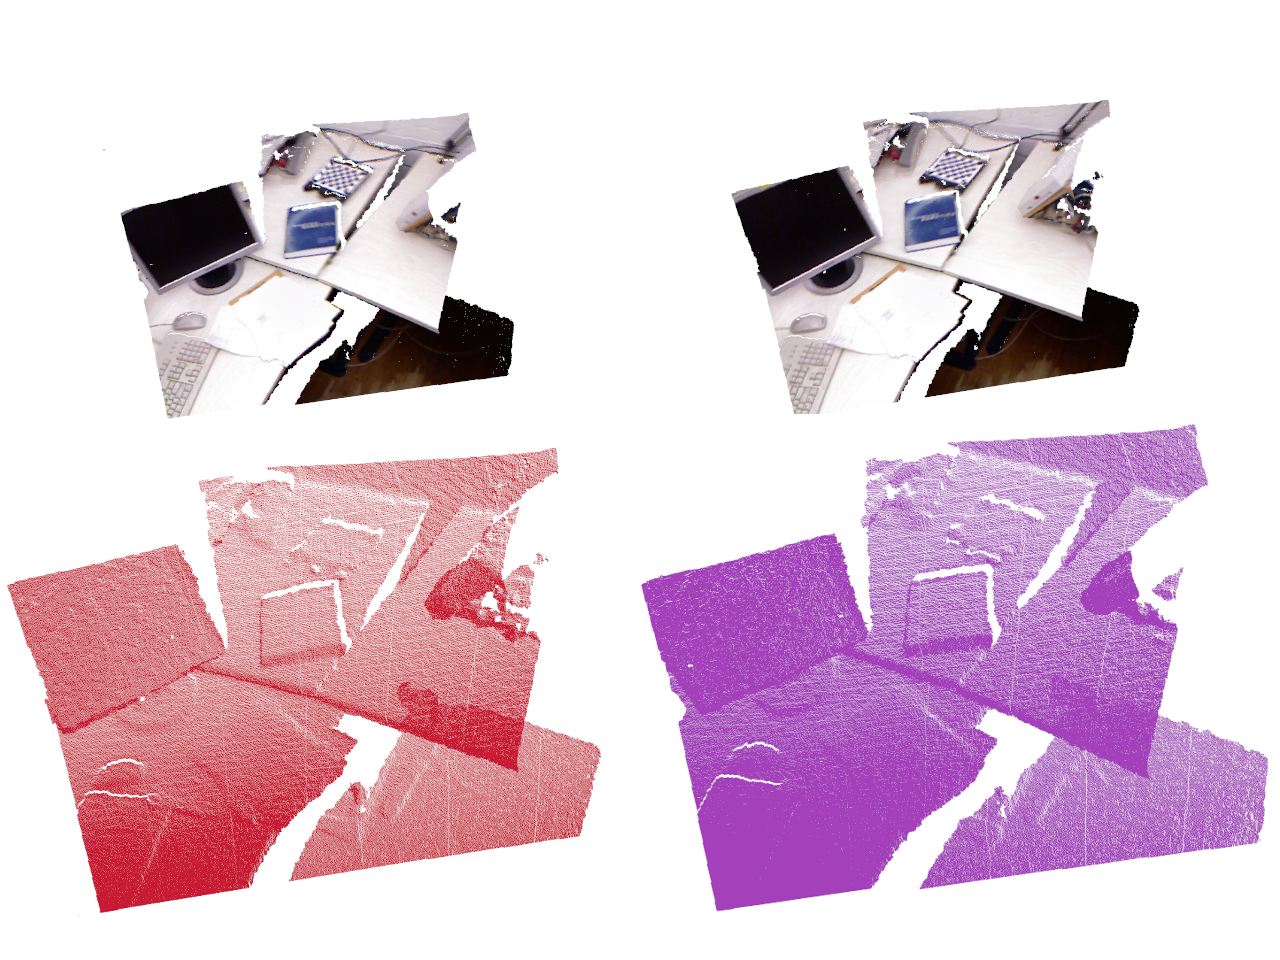
\includegraphics[scale=0.35]{images/two_clouds}
\caption{Two point clouds corresponding to a real life scene. We want to find the correct rotation and translation to align both point clouds.}
\end{center}
\end{figure}

